\phantomsection
\definecolor{dkgreen}{rgb}{0,0.6,0}
\definecolor{gray}{rgb}{0.5,0.5,0.5}
\definecolor{mauve}{rgb}{0.58,0,0.82}


\lstset{frame=tb,
language=R,
aboveskip=3mm,
belowskip=3mm,
showstringspaces=false,
columns=flexible,
numbers=none,
inputencoding=utf8/latin1,
keywordstyle=\color{blue},
numberstyle=\tiny\color{gray},
commentstyle=\color{dkgreen},
stringstyle=\color{mauve},
breaklines=true,
breakatwhitespace=true,
tabsize=3
}

\chapter{Introduzione}

Si possono ottenere le caratteristiche di una popolazione limitata mediante l'osservazione della totalità delle entità della popolazione o di un suo sottoinsieme, denominato "campione". Nel caso di una popolazione illimitata, è possibile lo studio solo mediante un campione di questa. Lo scopo dell'inferenza statistica è quello di estendere le misure ottenute dall'analisi di un campione a tutta la popolazione di cui il campione fa parte, accertandosi che il campione sia idoneo e rappresentativo per la popolazione.

L'\textit{inferenza statistica} si basa su due metodi fondamentali di indagine:

\begin{itemize}
    \item \textit{stima dei parametri}
    \item \textit{verifica delle ipotesi}
\end{itemize}

La \textit{stima dei parametri} ha lo scopo di determinare i valori non noti dei parametri di una popolazione, cioè il valore medio e la varianza, impiegando i parametri corrispondenti ottenuti dal campione. Questi parametri possono essere stimati utilizzando le \textit{stime puntuali} o le \textit{stime per intervallo}.

Per quanto riguarda la verifica delle ipotesi, consiste nella realizzazione di un'ipotesi sul parametro non noto e decidere la sua accettabilità in base ai risultati ottenuti dal campione estratto.

Per sfruttare l'inferenza statistica, l'analisi verterà sullo studio di un campione di una popolazione avente distribuzione normale. Si noti che R mette a disposizione per ogni distribuzione le seguenti funzioni:

\begin{itemize}
    \item $d$ calcola la funzione di probabilità di una variabile aleatoria in uno specifico punto o in un insieme di punti (density mass);
    \item $p$ calcola la funzione di distribuzione di una variabile aleatoria in uno specifico punto o in un insieme di punti (probability distribution);
    \item $q$ calcola la funzione quantili;
    \item $r$ simula una variabile aleatoria mediante la generazione di numeri pseudocasuali.
\end{itemize}

\section{Variabile Aleatoria Normale}

Nelle variabili aleatorie casuali continue è importante conoscere la probabilità che uno specifico valore sia compreso in un determinato intervallo.

\noindent \textbf{Definizione:} Una variabile aleatoria X di densità di probabilità

\[f_X(x) = \frac{1}{\sigma \sqrt{2\pi}}e^{-\frac{(x-\mu)^2}{2\sigma^2}}, \quad x \in \mathbb{R}, \quad (\mu \in \mathbb{R}, \sigma \> 0) \]

si dice avente distribuzione normale o di Gauss, di parametri $\mu$ (valore medio) e $\sigma$ (deviazione standard), principalmente utilizzata per la descrizione di fenomeni fisici e biologici.

La notazione del tipo $X ~ N(\mu, \sigma)$ indica che la $X$ ha distribuzione normale dei parametri $\mu$ e $\sigma$, o più semplicemente che è una variabile normale. Ci sono alcune proprietà che vengono soddisfatte dalla densità di probabilità normale, che sono:

\begin{itemize}
    \item simmmetria rispetto all'asse $x = \mu \forall x \in \mathbb{R} fx(\mu - x) = fx(\mu + x)$
    \item massimo nel punto di ascissa $x = \mu$ e nello specifico in $(\sigma \sqrt{2\pi})^{-1}$
    \item due punti di flesso nei punti $(\mu - \sigma)(\mu + \sigma)$
\end{itemize}

In R il calcolo della densità di probabilità di una variabile 
$X ~ N(\mu, \sigma)$ si può calcolare tramite la funzione \textit{dnorm}, la quale accetta come valori:

\begin{itemize}
    \item x, valori assunti dalla variabile aleatoria normale;
    \item mean e sd sono rispettivamente il valore medio e la deviazione standard della densità normale;
\end{itemize}

Il codice di seguito mostra come ottenere la densità di probabilità di una variabile aleatoria normale:

\vspace{5mm}
\begin{lstlisting}
  curve(dnorm(x, mean = -3, sd = 1),
        from = -6, to = 6, xlab = "x", ylab = "f(x)",
        main = " mu = [-3, -2, -1, 0, 1, 2, 3]; sigma = 1")
  curve(dnorm(x, mean = -2, sd = 1),
        from = -6, to = 6, xlab = "x",
        ylab = "f(x)", add = TRUE)
  curve(dnorm(x, mean = -1, sd = 1),
        from = -6, to = 6, xlab = "x",
        ylab = "f(x)", add = TRUE)
  curve(dnorm(x, mean = 0, sd = 1),
        from = -6, to = 6, xlab = "x",
        ylab = "f(x)", add = TRUE, lty = 2)
  curve(dnorm(x, mean = 1, sd = 1),
        from = -6, to = 6, xlab = "x",
        ylab = "f(x)", add = TRUE)
  curve(dnorm(x, mean = 2, sd = 1),
        from = -6, to = 6, xlab = "x",
        ylab = "f(x)", add = TRUE)
  curve(dnorm(x, mean = 3, sd = 1),
        from = -6, to = 6, xlab = "x",
        ylab = "f(x)", add = TRUE)
\end{lstlisting}
\vspace{5mm}

\begin{figure}[!htb]
    \centering
    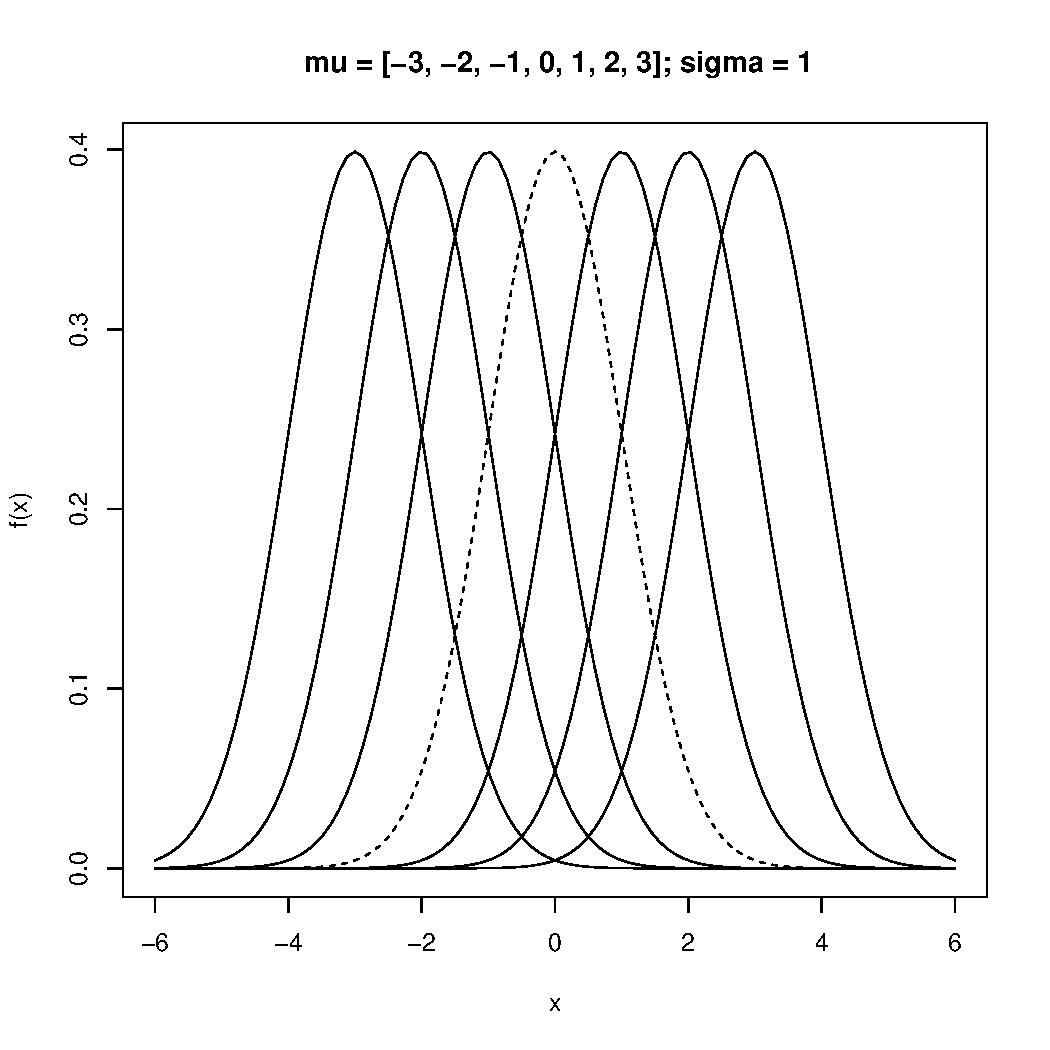
\includegraphics[height=16cm]{capitoli/images/1_introduzione/dens_prob_val.pdf}
    \caption{Densità normale.}
\end{figure}

Le variazioni al parametro $\mu$ comportano la traslazione della curva lungo tutto l'asse delle ascisse, senza cambiare la propria forma, mentre il parametro $\sigma$ caratterizza la larghezza della funzione. Poiché la massima ordinata è inversamente proporzionale a $\sigma$, decresce al crescere di $\sigma$ stesso mentre l'area sottesa della curva deve rimanere unitaria.

Quando $\mu = 0$ e $\sigma = 1$ possiamo ottenere la \textit{variabile aleatoria normale standardizzata.}

\vspace{5mm}
\begin{lstlisting}
  curve( dnorm(x,mean=0,sd=1), from=-6, to=6, xlab="x", ylab="f(x)", main="mu= 0, sigma=1")
\end{lstlisting}
\vspace{5mm}

\begin{figure}[!htb]
    \centering
    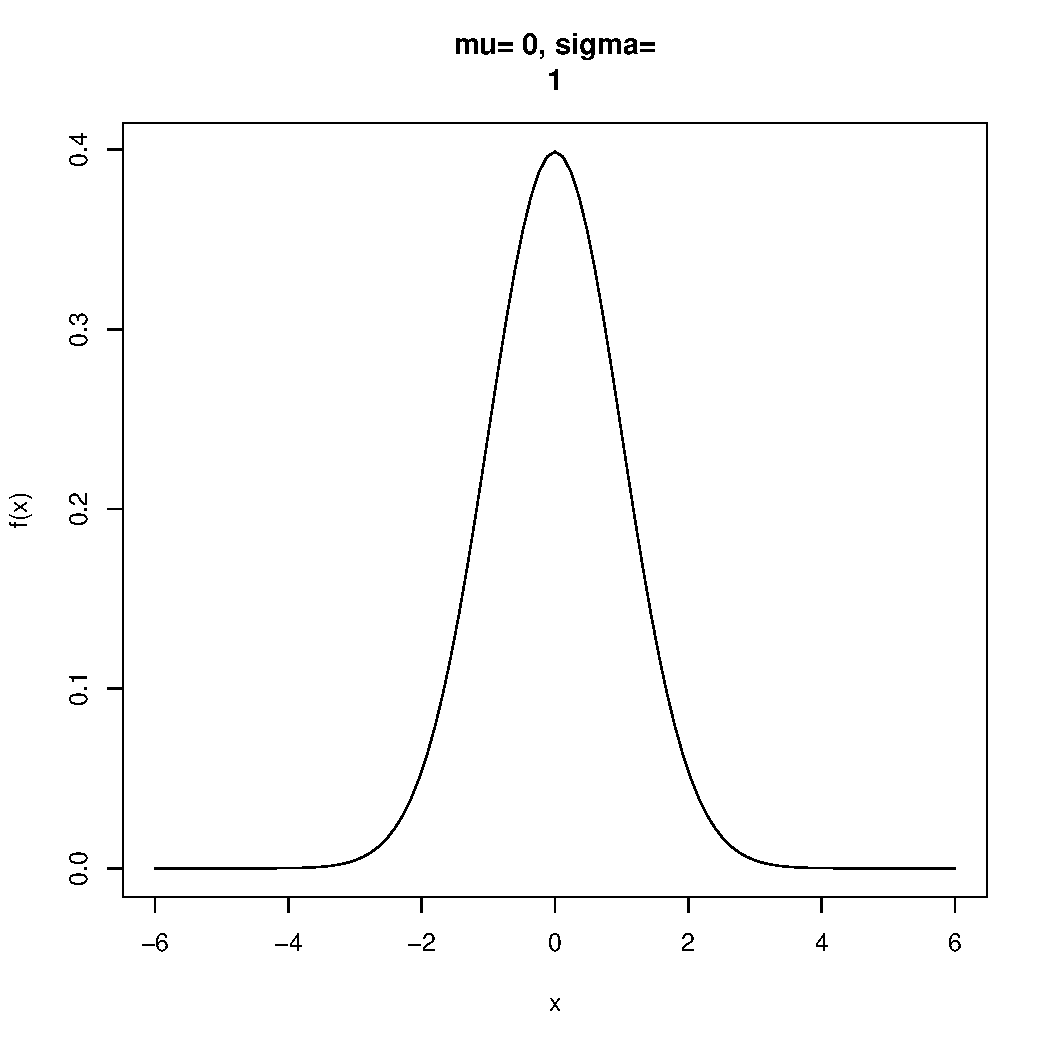
\includegraphics[height=16cm]{capitoli/images/1_introduzione/var_norm_stand.pdf}
    \caption{Variabile normale standard.}
\end{figure}

La funzione di distribuzione standard di uan variabile aleatoria $X ~ N(\mu, \sigma)$ è:

\[F_x(x) = P(X \leq x) = \int_{-\inf}^{x}fx(y)dy = \phi(\frac{x - \mu}{\sigma}) \quad x \in \mathbb{R}\]

dove 

\[\phi(z) = \frac{1}{\sqrt{2\pi}} \int_{-\inf}^z exp\{-\frac{y^2}{2}\}dy \quad z \in \mathbb{R}\]

è la funzione di distribuzione di una variabile aleatoria $Z ~N (0, 1)$

In R la funzione di distribuzione di una variabile $X \sim N(\mu, \sigma)$ può essere calcolata mediante l'impiego della funzione \textit{pnorm} la quale accetta come valori:

\begin{itemize}
    \item x, valori assunti dalla variabile aleatoria normale;
    \item mean e sd sono rispettivamente il valore medio e la deviazione standard della densità normale;
    \item lower.tail se TRUE calcola $P(X\leq x)$, se FALSE calcola $P(X \> x)$;
\end{itemize}

Il seguente codice mostra la funzione di distribuzione di una variabile aleatoria normale standard:

\vspace{5mm}
\begin{lstlisting}
  curve(pnorm(x, mean = 0, sd = 1), from = -4, to = 4, xlab = "x",
        ylab = expression(P(X <= x)), main = " mu = 0; sigma = 1", lty = 2)
  curve(pnorm(x, mean = 0, sd = 1), add = TRUE)
\end{lstlisting}
\vspace{5mm}

\begin{figure}[!htb]
    \centering
    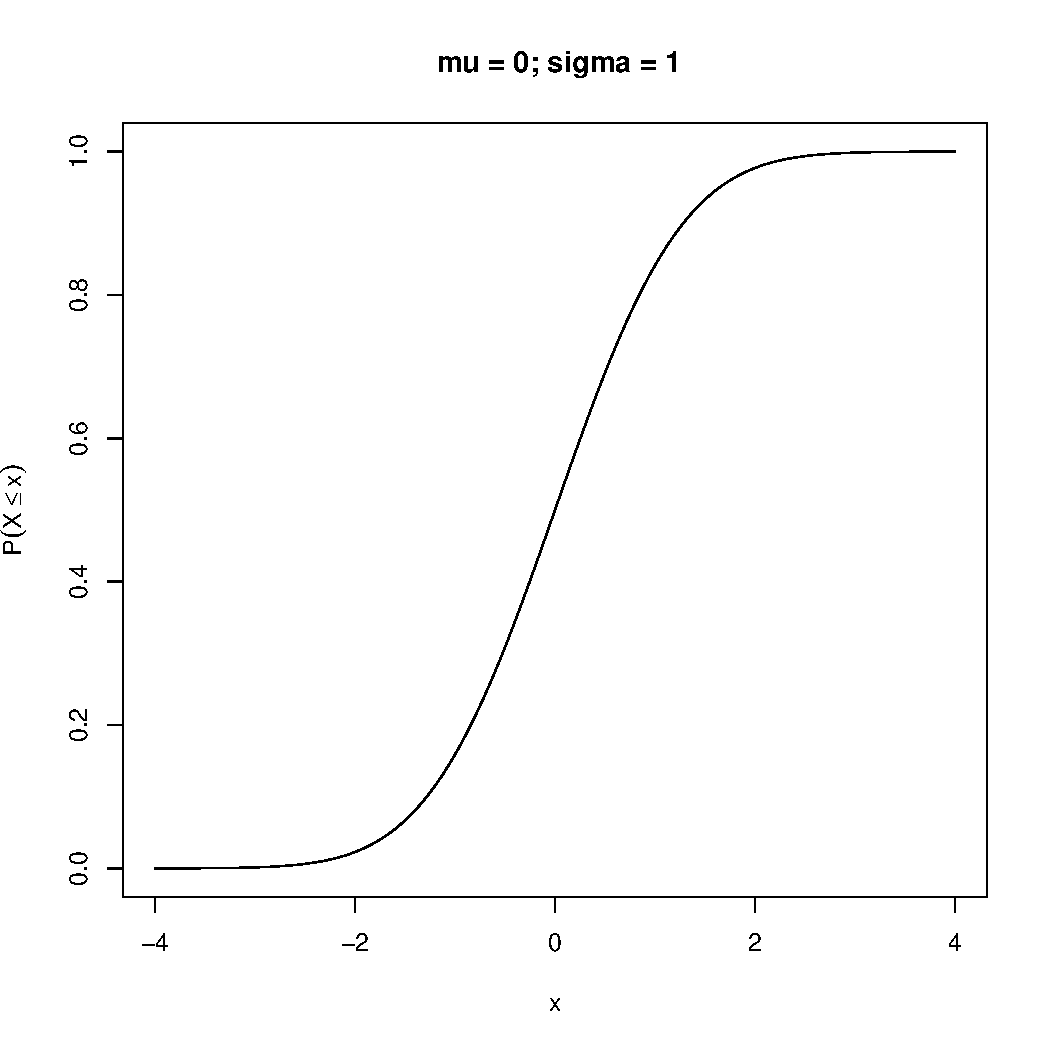
\includegraphics[height=16cm]{capitoli/images/1_introduzione/dist_var_norm_stand.pdf}
    \caption{Funzione di distribuzione della normale standard.}
\end{figure}


\section{Generazione del dataset}

Per generare il dataset si è utilizzata la funzione \textit{rnorm}.

\vspace{5mm}
\begin{lstlisting}
ds <- rnorm(80, 2, 0.5)

 [1] 2.5889415 2.4274552 2.2879886 2.5257274 1.3608815 1.8330865 2.2110392
 [8] 2.9302882 2.1603784 2.8153400 1.2379034 1.3232095 1.5533711 1.1738130
[15] 1.1798547 2.0803117 1.4592185 1.5569350 1.4902865 2.0316545 2.4187870
[22] 2.5316882 3.0833015 1.8875859 1.5517724 3.0869650 2.1161441 2.2039643
[29] 1.0669755 2.0200946 2.5388058 2.3822110 2.1206882 1.6142661 2.3803540
[36] 2.4263595 2.8091048 1.5316683 1.6807372 2.7404029 1.5801006 1.8411243
[43] 1.9379254 2.2090764 1.8581314 2.2168108 2.4149075 1.8682822 2.4080365
[50] 2.5663934 1.7010245 1.8328371 1.9498204 1.5384879 1.6274098 2.4448616
[57] 1.6637135 3.1919928 1.2788193 1.6247899 1.8259281 2.1353790 2.0575756
[64] 2.2415920 2.6733718 1.0493558 1.7638138 2.3932882 1.8392844 2.2664697
[71] 1.8736283 1.3277308 1.8608656 2.1320640 1.3944918 1.5087226 2.2219716
[78] 0.9680605 2.1960015 1.8015670
\end{lstlisting}
\vspace{5mm}

In questo caso è stato generato un campione formato da 80 elementi con $\mu = 2$ e $\sigma = 0.5$.
Ovviamente si suppone che il seguente campione sia stato estratto dalla popolazione e che esso sia rappresentativo di quest'ultima. Del dataset appena creato se ne calcola il valore medio $\mu$ e la deviazione standard $\sigma$.

\vspace{5mm}
\begin{lstlisting}
mu <- round(mean(ds), digits = 2)
mu
[1] 2

sigma <- round(sd(ds), digits = 2)
sigma
[1] 0.51
\end{lstlisting}
\vspace{5mm}

Una volta calcolati tali valori è possibile disegnare la variabile aleatoria normale che approssima il nostro campione attraverso la funzione dnorm:

\vspace{5mm}
\begin{lstlisting}
  curve(dnorm(x, mean = mu, sd = sigma), from = 0, to = 10, xlab = " x", ylab = "f(x)",
        main = paste("mu: ", mu, " sigma: ", sigma))
  lines(x = c(mu - sigma, mu, mu + sigma), y = dnorm(c(mu - sigma, mu, mu + sigma), mu, sigma),
        type = "h", lty = 2, col = c("green", "red", "green"), xlab = "")
  axis(1, at = c(mu - sigma, mu, mu + sigma), c("(mu - sigma)", "mu", "(mu + sigma)"))
\end{lstlisting}
\vspace{5mm}

\begin{figure}[!htb]
    \centering
    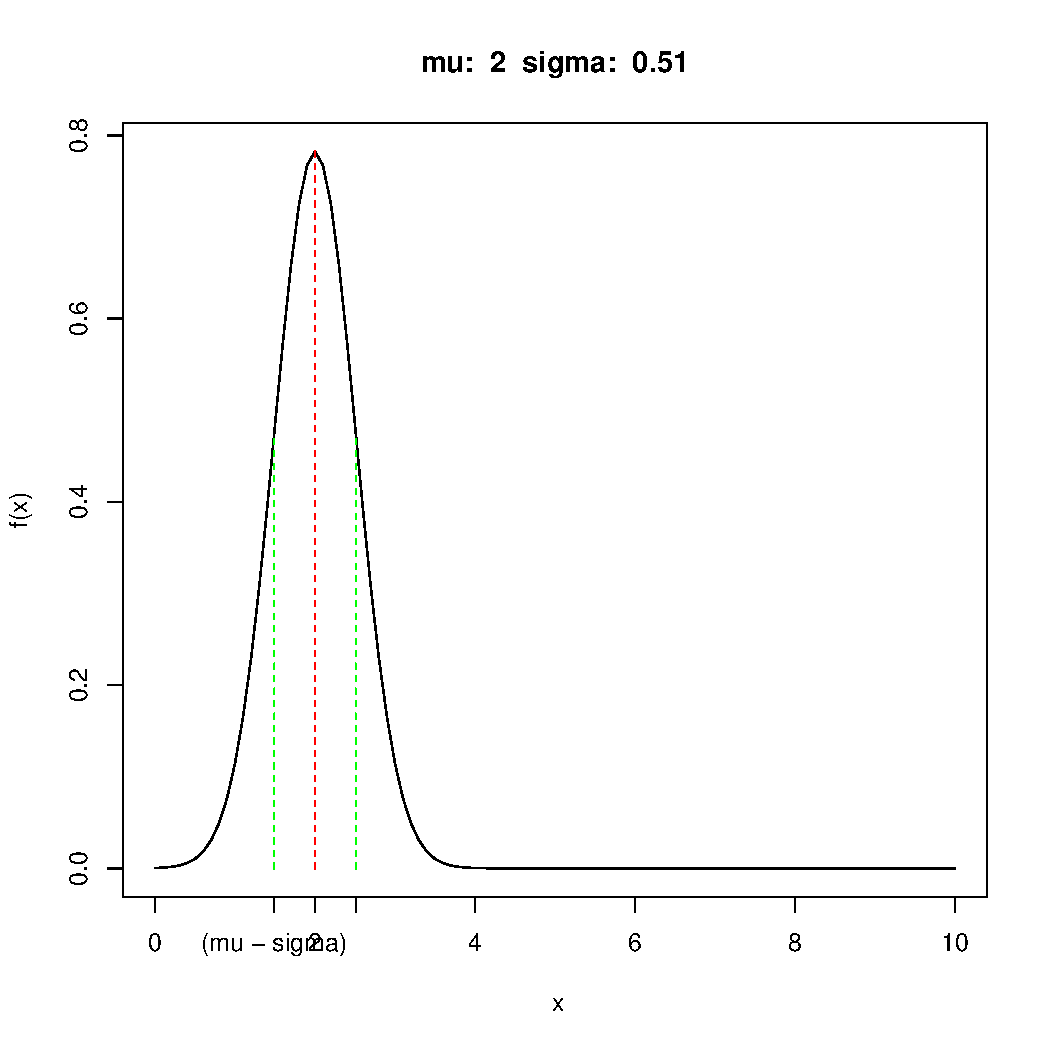
\includegraphics[height=16cm]{capitoli/images/1_introduzione/appross_dataset_norm.pdf}
    \caption{Approssimazione del dataset con la normale.}
    \label{app_data_norm}
\end{figure}

ottenendo la \ref{app_data_norm}, nella quale sono stati evidenziati in rosso il valore medio $\mu$ e in verde i due punti di flesso $(\mu - \sigma)$ e $(\mu + \sigma)$.






%################################################

\newpage